\documentclass[12pt]{article}
\usepackage[latin1,utf8]{inputenc}
\usepackage[brazil]{babel}
\usepackage{setspace}
\usepackage{boxedminipage}
\usepackage{latexsym}
\usepackage{multirow}
\usepackage[pdftex]{graphicx}
\usepackage{float}
\usepackage{url}
\usepackage{xcolor,listings}
\usepackage{amsmath}
\usepackage{biblatex}
\addbibresource{references.bib}

%\setlength{\parskip}{0.1cm}
\setlength{\paperheight}{29.7cm}
\setlength{\textheight}{23.0cm}
\setlength{\textwidth}{16.5cm}
\setlength{\oddsidemargin}{0.0cm}
\setlength{\topmargin}{-1.0cm}
\pagestyle{empty}

% Custom colors
\usepackage{color}
\definecolor{deepblue}{rgb}{0,0,0.5}
\definecolor{deepred}{rgb}{0.6,0,0}
\definecolor{deepgreen}{rgb}{0,0.5,0}

\begin{document}

\lstset{language=python,
    keywordstyle=\color{deepblue}\bfseries,
    commentstyle=\color{deepgreen},
    stringstyle=\ttfamily\color{deepred!50!brown},
    breaklines=true,
    showstringspaces=false}
\lstset{literate=%
   *{0}{{{\color{red!20!violet}0}}}1
    {1}{{{\color{red!20!violet}1}}}1
    {2}{{{\color{red!20!violet}2}}}1
    {3}{{{\color{red!20!violet}3}}}1
    {4}{{{\color{red!20!violet}4}}}1
    {5}{{{\color{red!20!violet}5}}}1
    {6}{{{\color{red!20!violet}6}}}1
    {7}{{{\color{red!20!violet}7}}}1
    {8}{{{\color{red!20!violet}8}}}1
    {9}{{{\color{red!20!violet}9}}}1
}

\begin{center}
{\sf {\large Visão e Processamento de Imagens - Avaliação única -
    Parte II}}

\textbf{Preste atenção para as regras da prova}
\end{center}
1- O fonte latex (.tex) da prova será disponibilizado para facilitar
que você não tenha que copiar o enunciado das questões. Todas as questões
devem ser respondidas no mesmo arquivo.

\noindent 2- A prova é \textbf{individual}.  É permitido a consulta a
livros, apontamentos ou Internet, desde que devidamente referenciada.
Não é permitida a consulta a colegas, amigos, família, cachorro,
papagaio e etc. 

\noindent 3- A prova deve ser entregue diretamente no Paca, assim como
todos os códigos e imagens devem ser entregues no mesmo arquivo
comprimido.  \textbf{Duração da prova: 14 dias}.  

\noindent 4- Cada questão vale 20 pontos (pois são apenas 3 questões)
para a graduação e 15 pontos para a pós-graduação (pois são 4 questões). 
\bigskip

\begin{itemize}
\item[{\bf Q1.}] Para fazer esta questão, leia primeiro o artigo abaixo:
\begin{itemize}
\item \url{http://www.eecs.berkeley.edu/Pubs/TechRpts/2015/EECS-2015-85.pdf}
\end{itemize} 
\begin{itemize}
\item Faça um resumo do artigo de acordo com as indicações que deixei no paca (artigos sobre como fazer um resumo).

\textbf{TODO}

\item Implemente o método ELA (Error Level Analysis) em Python (apresente o 
\textbf{algoritmo} na prova e anexe o código em Python no arquivo zip).

Abaixo o trecho onde o algoritmo efetivamente foi implementado. O código completo está em \textbf{source/ela.py}.
    
\begin{lstlisting}[basicstyle=\ttfamily]
import os
from PIL import Image, ImageChops, ImageEnhance
from time import gmtime, strftime

# you can change the image directory here
HOAX_IMAGES = './HoaxImages/'

def check_image(img_path, scale=20.0, show=False):
    """ Compute the Error Level Analysis for the given image
    
    Save a copy of the given image changing its quality level,
    in our case 95%, and compute the difference between this 
    image over the original. In addition, a scale is also 
    applied to the final result for better viewing.
    
    References: 
    http://blackhat.com/presentations/bh-dc-08/Krawetz/Whitepaper/bh-dc-08-krawetz-WP.pdf
    http://www.eecs.berkeley.edu/Pubs/TechRpts/2015/EECS-2015-85.pdf
    """
    try:
        img = Image.open(img_path)
    except FileNotFoundError:
        print ("File '"+ img_path +"' not found.")
        return
    
    # check the image format for JPEG only
    if img.format is not 'JPEG':
        log(img_path + ' is not a JPEG file')
        return

    log("Image size "+ str(img.size[0]) + "x" + str(img.size[1]))
    short_file_name = os.path.splitext(img_path)[0]
    
    # save a copy of the image with a different inferior quality level
    resaved_path = short_file_name + '_resaved'
    img.save(resaved_path, 'JPEG', quality=95)
    resaved_img = Image.open(resaved_path)
    
    # compute the difference between the given image and the image
    # generated applying a scale to increase the brightness
    ela_img = ImageChops.difference(img, resaved_img)
    ela_img = ImageEnhance.Brightness(ela_img).enhance(scale)
    ela_img.save(short_file_name + '_ela.png')
    if (show):
        ela_img.show()
    
    os.remove(resaved_path)
\end{lstlisting}

\item Teste seu algoritmo com as imagens que deixei no paca para este exercício. 
Quantas imagens seriam consideradas modificadas por esse método? Comente o resultado,
comparando com a sua intuição.

Uma vez submetida a imagem ao \textit{Error Level Analysis}, pode-se perceber pelo resultado que 
a região manipulada terá um nível de erro diferente das regiões não manipuladas. Logo, 
o nível de erro irá expor a região manipulada rotulando as regiões com maior alteração após
a imagem ser salva com um nível de qualidade inferior \cite{krawetz}.

Na Figura 1b, podemos ver o resultado do ELA na imagem dada. As regiões com maior chance de ter
alterações são as que apresentam os pixels com maior brilho, uma vez que a alteração da imagem 
causa instabilidade nestas áreas.
\begin{figure}[htb]
\centering
\begin{minipage}[b]{0.45\textwidth}
	\centering
        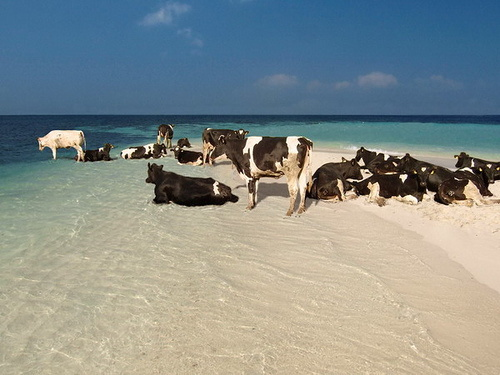
\includegraphics[scale=0.3]{Q3Images/cows_on_beach.jpg} 
	\centerline{\label{fig1a} \small (1a) Imagem original}
\end{minipage}
\begin{minipage}[b]{0.45\textwidth}
	\centering
        
\includegraphics[scale=0.3]{Q3Images/cows_on_beach_ela.png} 
	\centerline{\label{fig1b} \small (1b) Imagem com o resultado do ELA}
\end{minipage}
\end{figure}

Os resultados foram avaliados de acordo com o brilho das bordas que devem ser semelhantes no resultado 
da aplicação do ELA na imagem. Além disso, regiões de cores e texturas semelhantes na imagem
original, independentemente da cor, também devem ter cores aproximadamente similares no ELA \cite{berkeleywebsite}.

Isto posto, um total de 23 imagens foram consideradas alteradas de acordo com o método e avaliação a posteriori.
\end{itemize}
%
%
%
\item[{\bf Q2.}] Esta questão refere-se à transformada de Fourier.
\begin{itemize}
\item Encontre a transformada de Fourier da função:
\begin{eqnarray*}
f(x) = \left\{ \begin{array}{rl} 
 7 &\mbox{ if $-5 < x < 5$} \\
 0 &\mbox{ caso contrário}
       \end{array} \right.
\end{eqnarray*}

Por definição, temos que a transformada de Fourier de um pulso
retangular de largura $D$ e altura $A$ tem a forma dada por:

\begin{eqnarray*}
    F(\omega) = ADsinc(\frac{\omega D}{2})  = AD\frac{sin(\frac{\omega D}{2})}{\frac{\omega D}{2}}
\end{eqnarray*}

A função $f(x)$ pode ser representada graficamente como:
\begin{figure}[htb]
\centering   
\begin{minipage}[b]{0.45\textwidth}
	\centering
        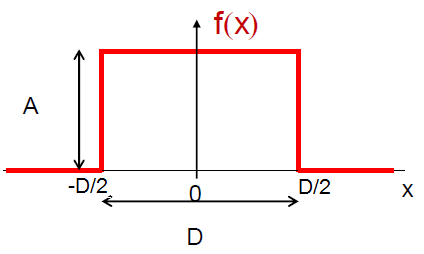
\includegraphics[scale=0.3]{Q3Images/pulse_function.png} 
\end{minipage}
\end{figure}

Onde:
\begin{eqnarray*}
f(x) = \left\{ \begin{array}{rl} 
 A, &\mbox{ $x \in  [\frac{-D}{2}, \frac{D}{2}]$} \\
 0, &\mbox{ $x \notin [\frac{-D}{2}, \frac{D}{2}]$}
       \end{array} \right.
\end{eqnarray*}

Logo, temos que A = 7 e D = 10 e, portanto, a transformada de Fourier da função $f(x)$ é:
\begin{eqnarray*}
    F(\omega) = AD\frac{sin(\frac{\omega D}{2})}{\frac{\omega D}{2}} \
              = 7*10\frac{sin(\frac{\omega 10}{2})}{\frac{\omega 10}{2}} \
              = 70\frac{sin(\frac{\omega 10}{2})}{\frac{\omega 10}{2}} \
              = 70\frac{sin(5\omega)}{5\omega}
\end{eqnarray*}

%%%
\item Encontre a transformada de Fourier da função $ g(x) = f(x)\cos
   \omega_0 x$, sabendo que a transformada de Fourier de $f(x)$ é dada
   por $F(\omega)$


\item Ache a inversa da transformada de Fourier de $G(\omega) =
  20\frac{\sin 5\omega}{5\omega}e^{-3\omega i}$
  
\textbf{TODO}
\item Calcule a DFT do sinal $f = \{1,3,5,3,1\}$

A DFT é dada por:
\begin{align*}
    F(k) = \sum\limits_{n=0}^{N-1} f(n) e^{-jk\frac{2\pi}{N}n}
\end{align*}

Para realizar os cálculos devemos utilizar a identidade de Euler:
\begin{align*}
    e^{-j \pi} = \cos \pi - j\sin\pi
\end{align*}
Devemos utilizar a seguinte equação para calcular a DFT do sinal dada:
\begin{align*}
    X[k] = \sum\limits_{n=0}^{N-1} x[n] e^{-jk\frac{2\pi}{N}n},\qquad para\quad k=0,1,2,...,N-1
\end{align*}
Temos que N=5, logo:
\begin{align*}
    &X[0] = (1e^0 + 3e^0 + 5e^0 + 3e^0 + 1e^0) &\\
    &X[1] = (1e^0 + 3e^{-j1\frac{2\pi}{5}1} + 5e^{-j1\frac{2\pi}{5}2} + 3e^{-j1\frac{2\pi}{5}3} + 1e^{-j1\frac{2\pi}{5}4)} &\\
    &X[2] = (1e^0 + 3e^{-j2\frac{2\pi}{5}1} + 5e^{-j2\frac{2\pi}{5}2} + 3e^{-j2\frac{2\pi}{5}3} + 1e^{-j2\frac{2\pi}{5}4)} &\\
    &X[3] = (1e^0 + 3e^{-j3\frac{2\pi}{5}1} + 5e^{-j3\frac{2\pi}{5}2} + 3e^{-j3\frac{2\pi}{5}3} + 1e^{-j3\frac{2\pi}{5}4)} &\\
    &X[4] = (1e^0 + 3e^{-j4\frac{2\pi}{5}1} + 5e^{-j4\frac{2\pi}{5}2} + 3e^{-j4\frac{2\pi}{5}3} + 1e^{-j4\frac{2\pi}{5}4)} &\\
    &X[0] = (1 + 3 + 5 + 3 + 1) &\\
    &X[1] = (1 + 3e^{-j\frac{2\pi}{5}} + 5e^{-j\frac{4\pi}{5}}  + 3e^{-j\frac{6\pi}{5}}  + 1e^{-j\frac{8\pi}{5})} &\\
    &X[2] = (1 + 3e^{-j\frac{4\pi}{5}} + 5e^{-j\frac{6\pi}{5}}  + 3e^{-j\frac{12\pi}{5}} + 1e^{-j\frac{16\pi}{5})} &\\
    &X[3] = (1 + 3e^{-j\frac{6\pi}{5}} + 5e^{-j\frac{12\pi}{5}} + 3e^{-j\frac{18\pi}{5}} + 1e^{-j\frac{24\pi}{5})} &\\
    &X[4] = (1 + 3e^{-j\frac{8\pi}{5}} + 5e^{-j\frac{16\pi}{5}} + 3e^{-j\frac{24\pi}{5}} + 1e^{-j\frac{32\pi}{5})}&
\end{align*}
Calculando cada componente com a relação de Euler e substituindo os resultados na equação acima:
\begin{align*}
    &e^{-j\frac{2\pi}{5}} = cos(\frac{2\pi}{5}) - jsen(\frac{2\pi}{5}) = 0,30902  - 0,95106j &\\
    &e^{-j\frac{4\pi}{5}} = cos(\frac{4\pi}{5}) - jsen(\frac{4\pi}{5}) = -0,80902 - 0,58779j &\\
    &e^{-j\frac{6\pi}{5}} = cos(\frac{6\pi}{5}) - jsen(\frac{6\pi}{5}) = -0,80902 + 0,58779j &\\
    &e^{-j\frac{8\pi}{5}} = cos(\frac{8\pi}{5}) - jsen(\frac{8\pi}{5}) = 0,30902  - 0,95106j &\\
    &e^{-j\frac{12\pi}{5}} = cos(\frac{12\pi}{5}) - jsen(\frac{12\pi}{5}) = 0,30902	-0,95106j &\\
    &e^{-j\frac{16\pi}{5}} = cos(\frac{16\pi}{5}) - jsen(\frac{16\pi}{5}) = -0,80902 + 0,58779j &\\
    &e^{-j\frac{18\pi}{5}} = cos(\frac{18\pi}{5}) - jsen(\frac{18\pi}{5}) = 0,30902 + 0,95106j &\\
    &e^{-j\frac{24\pi}{5}} = cos(\frac{24\pi}{5}) - jsen(\frac{24\pi}{5}) = -0,80902 - 0,58779j &\\
    &e^{-j\frac{32\pi}{5}} = cos(\frac{32\pi}{5}) - jsen(\frac{32\pi}{5}) = 0,30902	- 0,95106j&
\end{align*}
Temos então que o resultado da DFT é:
\begin{multline*}
    X[f] = 13, -4.236067-3.077683j, 0.236067+0.726542j, \\
           0.236067-0.726542j, -4.236067+3.077683j
\end{multline*}

\end{itemize}
%
%
%
\item[{\bf Q3.}] 
\begin{itemize}
\item Calcule (apresente os cálculos) dos descritores de Fourier das
  figuras 3a e 3b. Lembre-se que os pontos da
  borda do quadrado serão representados por pontos no plano de
  Argand-Gauss. Isto é, cada ponto no plano passa a ser um número
  complexo e a borda passa a ser um vetor de pontos complexos, como
  num sinal, mas com valores complexos.

\textbf{TODO}

\item Para confirmar que seus cálculos estão corretos, implemente um
  programa em Python que receba como entrada um vetor de números
  complexos (que são as coordenadas das bordas) e retorne os
  descritores de Fourier do vetor de entrada. Você pode usar as
  funções fornecidas pela biblioteca NUMPY para facilitar a
  programação.
  
\textbf{TODO}

\item Para reconstruir a curva, faça uma função que receba um vetor
  com os descritores de Fourier, um número $N$ de descritores a serem
  usados e grafique os pontos num plano cartesiano (para fazer a mesma 
figura que fizemos nos slides das aulas 15 e 16.

\textbf{TODO}

\end{itemize}
\begin{figure}[htb]
\centering
\begin{minipage}[b]{0.45\textwidth}
	\centering
        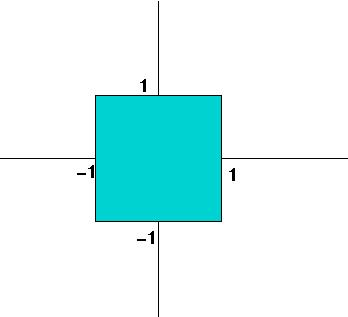
\includegraphics[scale=0.2]{Q3Images/square1.jpg} 
	\centerline{\label{fig3a} \small (3a) Quadrado de lado 1}
\end{minipage}
\begin{minipage}[b]{0.45\textwidth}
	\centering
        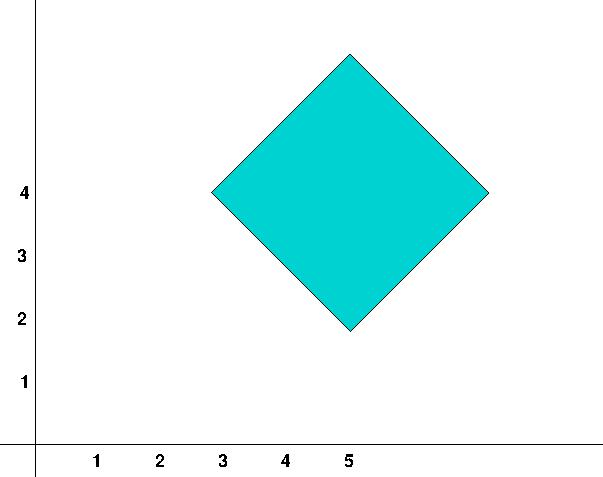
\includegraphics[scale=0.3]{Q3Images/square3.jpg} 
	\centerline{\label{fig3b} \small (3b) Quadrado de lado 3}
\end{minipage}
\end{figure}

%
%
%
\item[{\bf Q4.}] \textbf{Apenas para os alunos de pós-graduação} 
\begin{itemize}
\item Leia o artigo do Torre e do Poggio
  \url{ftp://publications.ai.mit.edu/ai-publications/pdf/AIM-768.pdf}
  e faça um resumo de acordo com as indicações que deixei no
  paca (artigos sobre como fazer um resumo). 
\item O que é um problema mal-posto?
\item O que é regularização? 
\item Qual a importância do teorema apresentado no artigo?
\item O que são filtros de banda limitada? Qual a sua importância no
  artigo?
\item Quais são os métodos de encontrar borda apresentados no artigo?
\end{itemize}
\end{itemize}

\printbibliography
\end{document}
